\documentclass[../main.tex]{subfiles}


\begin{document}
\section{Highest temperature of the year}
	The aim of this subproject was to obtain the highest temperature of the year for all available cities and compare them. In order to do this we created a function in the 
	main (project.cpp) file which reads in all of the city objects which is needed for the plotting in the end.
	\\\\
	The code uses one function which is part of the tempTrender class. The function uses a variable called ``highestTemperature'' which is used in order to determine 
	the highest temperature of the year. The variable is first put to a low temperature (0 celsius) as we know the highest temperature will guaranteed be higher than this. 
	The function then starts a for loop which goes over all the data points. If the temperature of the data point is higher than the highest temperature variable, it 
	replaces its value. At the end of each year the highest temperature and the current year is stored in two vectors before resetting the variable. This way one will obtain 
	the highest temperature of each year in an easily accessed vector.
	\\\\
	Next step of the subproject was to plot all of the results together in one plot in order to make comparisons easier. The plotting used a for loop and a pointer to reduce 
	the code length by avoiding nine sets of (x,y) lists declarations and value assignments. Figure \ref{highestTemperature2} shows the results of the subproject.
	\begin{figure}[H]
	  \centering
	  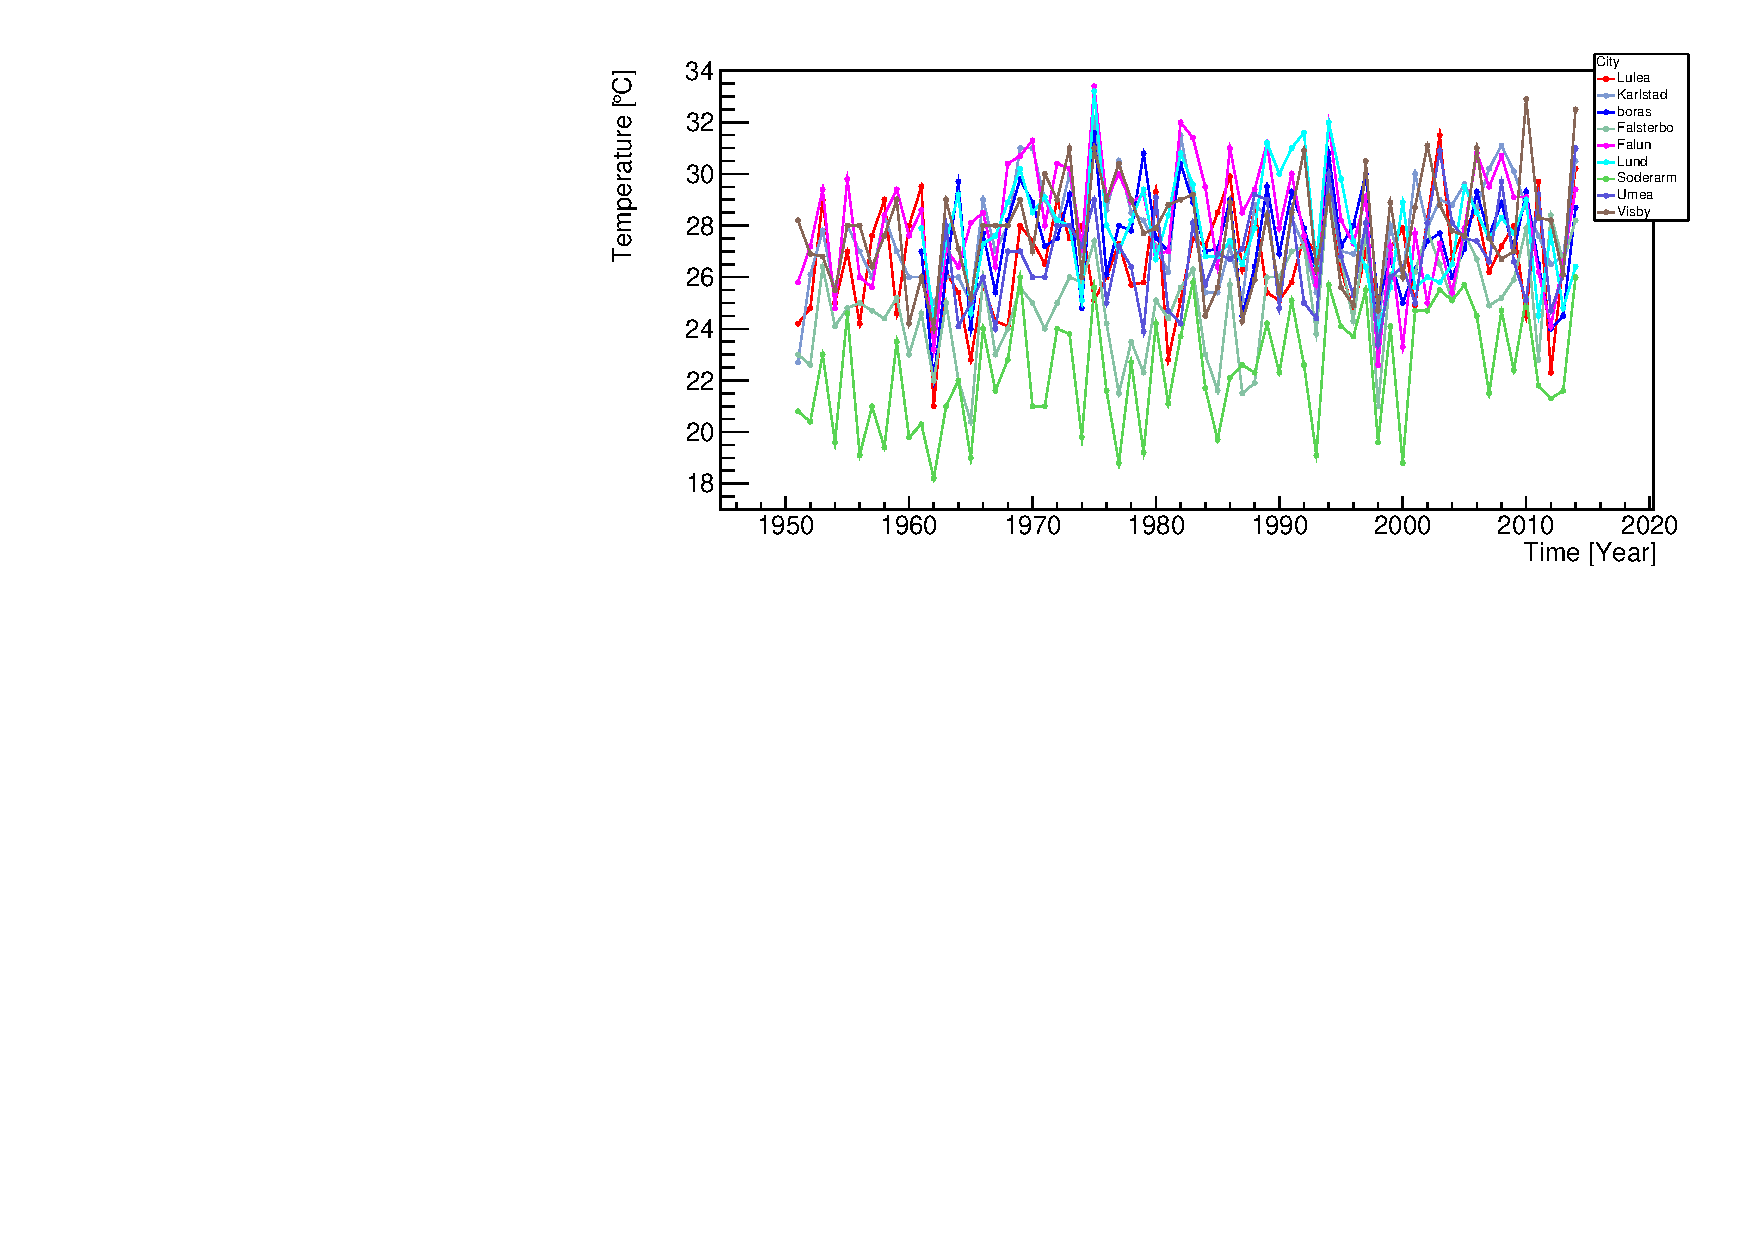
\includegraphics[width = \textwidth]{hottestdaysallcities}
	  \caption{Highest temperature per year for Borås, Falsterbo, Falun, Karlstad, Luleå, Lund, Söderarm, Umeå and Visby.}
	  \label{highestTemperature2}
	\end{figure}\noindent
	The results are very messy, however one can see that Söderarm is constantly at the bottom and for some years all of the cities have a raised temperature. It could have 
	been smart to split it up into two separate figures in order to increase readability.

\end{document}